\section[Word vectors]{From word counts to word vectors}


\begin{frame}{Our BOW approach until now}
  \begin{block}{Representing a document by word frequency counts}
    Result of preprocessing and vectorizing:
    
    0. \texttt{He took the dog for a walk to the dog playground}\\
    $\Rightarrow$ \texttt{took dog walk dog playground}\\
    $\Rightarrow$ \texttt{'took':1, 'dog': 2, walk: 1, playground: 1}
  \end{block}
  
  Consider these other sentences
  \begin{enumerate}
  \item<2-> He took the doberman for a walk to the dog playground
  \item<3-> He took the cat for a walk to the dog playground
  \item<4-> He killed the dog on his walk to the dog playground 
  \end{enumerate}
  
  \onslide<5>{The vectorized representations of these sentences have a ``distance'' (dissimilarity) of 1 each, but arguably, sentences 0 and 1 should be ``closer'' than others}
	
\end{frame}


\begin{frame}{Our BOW approach until now}
  \begin{itemize}
  \item Our vectorizers gave a random ID to each word
  \item What if we instead would represent each word by another vector representing its meaning?
  \item For, instance, `doberman' and `dog' should be represented by vectors that are close to each other in space, while `kill' and `walk' should be far from each other.
  \end{itemize}
  \pause
  $\Rightarrow$ That's the idea behind word embeddings!
  
  \pause
  
  Or, more broadly: Can computers understand meanings, semantic relationships, different types of contexts?
\end{frame}


\subsection{Training word embeddings}

\begin{frame}{GloVe vs Word2Vec}
  There are two popular approaches to training word embeddings: GloVe and word2vec.
  \begin{itemize}
  \item GloVe is count-based: dimensionality reduction on the co-occurrence count matrix.
  \item Word2Vec is a predictive model: neural network to predict words/contexts
  \item That means that GloVe takes \emph{global} context into account, word2vec \emph{local} context
  \item Some technical implications for how training can be implemented 
  \item \textbf{However, often only subtle differences in final result.}
  \end{itemize}
\end{frame}



\begin{frame}{Word2Vec: Continous Bag of Words (CBOW) vs skipgram}
  Example sentence: ``the quick brown fox jumped over the lazy dog''
  \begin{block}{CBOW: Predict a word given its context}
    Dataset:
    
    \texttt{([the, brown], quick), ([quick, fox], brown), ([brown, jumped], fox), ...}
  \end{block}
  
  \pause
  
  
  \begin{block}{skipgram: Predict the context given the word}	
    \texttt{(quick, the), (quick, brown), (brown, quick), (brown, fox), ...}
  \end{block}
  
  \tiny{Example taken from here: \url{https://medium.com/explore-artificial-intelligence/word2vec-a-baby-step-in-deep-learning-but-a-giant-leap-towards-natural-language-processing-40fe4e8602ba}}
\end{frame}

%window sizes


\begin{frame}{Continous Bag of Words (CBOW) vs skipgram}
  \begin{itemize}
  \item CBOW is faster
  \item skipgram works better for infrequent words
  \item Both are often used
  \item Usually, we use larger window sizes (e.g, 5)
  \item We need to specify the number of dimensions (typically 100--300)
  \end{itemize}
  \pause
  
  \textit{In any event, as a result of the prediction task, we end up with a \{100|200|300\}-dimensional vector representation of each word.*}
  
  
  \tiny{* If that makes you think of PCA/SVD, that's not completely crazy, see \cite{Levy2018}}\\
\end{frame}




\begin{frame}{``...a word is characterized by the company it keeps...''\parencite{Firth1957}}
  \begin{block}{Word embeddings \ldots}
    \begin{itemize}
    \item help capturing the meaning of text
    \item are low-dimensional vector representations that capture semantic meaning
    \item are very common in NLP...
    \end{itemize}
  \end{block}

\end{frame}

%Due to developments in the field of NLP, algorithms have become increasingly apt to understand human language. Word embeddings are the current state of the art for capturing the meaning of texts. Word embeddings are vector representations of words. They are the current state of the art in NLP to understand, capture and process language. The basic idea of word embeddings is that one gets to know a word by looking at the company that it keeps; contexts is crucial in understanding word meaning. 


\begin{frame}{You can literally calculate with words!}
	And answer questions such as ``Man is to woman as king is to \_\_\_\_?''
	\makebox[\linewidth]{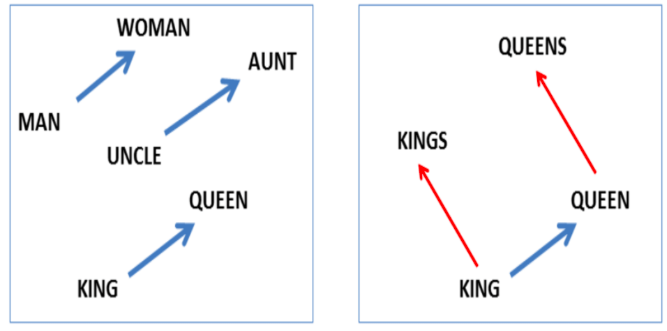
\includegraphics[width=\linewidth,height=\textheight, keepaspectratio]{embeddings.png}}
	semantic relationships vs. syntactic relationships
\end{frame}

%word vectors that are able to capture the relationships between words in a surprisingly expressive way. Word embeddings are especially effective in understanding analogies, and for example understand that man is to woman as uncle to aunt, and king to king. 



\subsection[Improving models]{Using word embeddings to improve models}

\question{What can we use word embeddings for?}

\begin{frame}{In supervised machine learning}
  \begin{itemize}[<+->]
  \item For instance, we could modify our vectorizer such that for each term, you do not only count how often it occurs, but also multiply with its embedding vector
  \item Aggregate these embeddings (e.g., sum or mean) and represent document with 300 instead of 10,000 dimensions!
  \item Often, pre-trained embeddings (e.g., trained on the whole wikipedia) are used
  \item Thus, our supervised model will be able to deal with synonyms and related words!
  \end{itemize}


  
  \pause 
  Let's look at an example for using supervised sentiment analysis (i.e., what we did with IMDB-data before).
  
	
\end{frame}



\begin{frame}{In classical SML:}
\begin{itemize}[<+->]
\item we represent each document by a vector of word frequencies (or tf$\cdot$ idf scores)
\item use these vectors to predict the label
\end{itemize}
\end{frame}


\begin{frame}[plain]
        	\begin{table}[]
	        	\resizebox{\textwidth}{!}{%
			\begin{tabular}{lllllllll}
				& ability & about & above & \ldots & zippered  & zealotry & $\rightarrow$ & \textcolor{orange}{topic} \\
				text1 & \ding{110}  & \ding{110}  &\ding{110}  & \ldots & \ding{110}  & \ding{110} & $\rightarrow$ &\textcolor{orange}{\ding{110}}  \\
				text2 & \ding{110}  & \ding{110}   &\ding{110} & \ldots  & \ding{110}  & \ding{110} & $\rightarrow$ &\textcolor{orange}{\ding{110}} \\
				text3 & \ding{110}  & \ding{110}   &\ding{110} & \ldots & \ding{110}  & \ding{110} & $\rightarrow$ &\textcolor{orange}{\ding{110}} \\
				text4 & \ding{110}  & \ding{110}  &\ding{110} & \ldots  & \ding{110}  & \ding{110} & $\rightarrow$ &\textcolor{orange}{\ding{110}} \\
				&&&&&&& \\
				new case & \ding{110}  & \ding{110}  & \ding{110}  & \ldots & \ding{110}  & \ding{110} & $\rightarrow$ &\textbf{\textcolor{orange}{?}} \\
			\end{tabular}%
		}
		\raggedright	
		For instance, topic can be [``sports'', ``economy'', ``politics''] and the other entries are word frequencies
	\end{table}
\end{frame}



\begin{frame}{The idea}
  We modify our vectorizer such that
  \begin{itemize}[<+->]
  \item for each word in the document, we look up its embedding
  \item we then aggregate these embeddings (e.g., mean, max, or sum)
  \item For each document, we now have a 300-dimensional instead of a 10,000-dimensional vector\footnote{in the case of a 300-dimensional embedding model and a vocabulary size of 10,000 of the traditional CountVectorizer)}
  \end{itemize}
\tiny{Example implementation at \url{https://github.com/ccs-amsterdam/embeddingvectorizer}}	
\end{frame}



\begin{frame}{What does that mean?}
	A couple of things:
	\begin{itemize}[<+->]
		\item Our model is smaller
		\item We can use words in the prediction dataset \emph{even if it's not in the training dataset}\footnote{as long as it's in the embedding model, of course}
		\item We can learn from similar training samples even if they do not use the same words
		\item But we also may loose some nuance
	\end{itemize}
\end{frame}




\begin{frame}{Let's look at an example}
	As we see, not \emph{all} embedding models are improving downstream tasks -- but good ones can:
	\url{https://github.com/annekroon/amsterdam-embedding-model}
	
	\instruction{explain results in README.md}
\end{frame}











\begin{frame}[plain]
  \makebox[\linewidth]{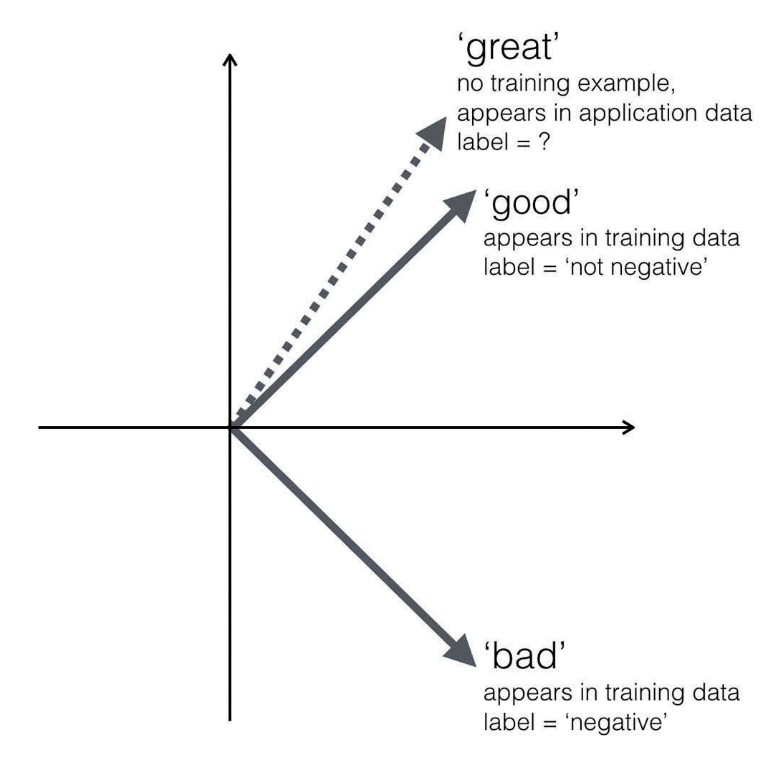
\includegraphics[width=\linewidth,height=\textheight, keepaspectratio]{rudkowsky2018-1}}
	

  \cite{Rudkowsky2018a}
\end{frame}


\begin{frame}{It's not always black/white\ldots}
	Sometimes, BOW may be just fine (for very negative sentences, it doesn't matter). But especially in less clear cases ('slightly negative'), embeddings increased performance.
	\makebox[\linewidth]{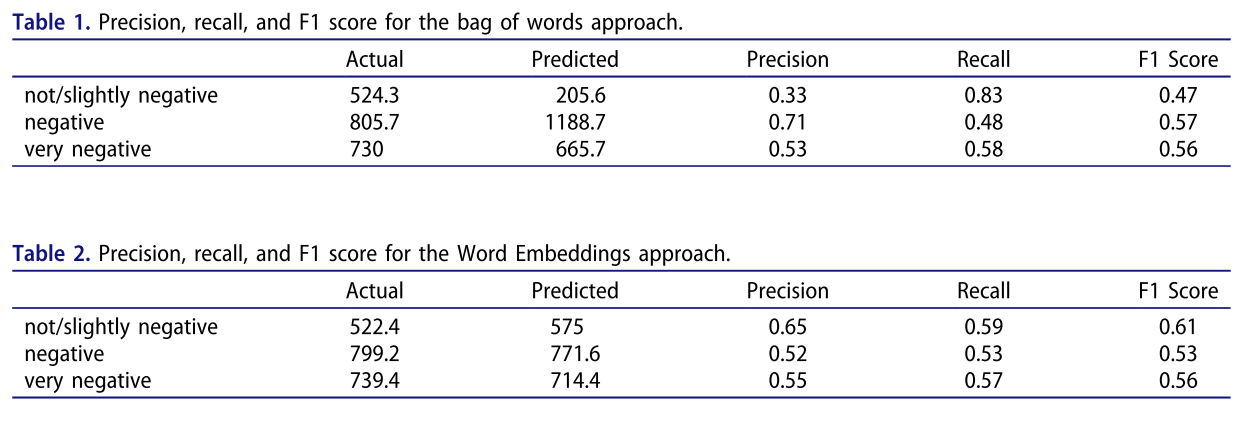
\includegraphics[width=\linewidth,height=\textheight, keepaspectratio]{rudkowsky2018-2}}
	
	\vfill
	\cite{Rudkowsky2018a}
\end{frame}


\subsection{Document similarity}

\begin{frame}{In document similarity calculation}
  \begin{block}{Use cases}
    \begin{itemize}
    \item plagiarism detection
    \item Are press releases/news agency copy/\ldots taken over?
    \item Event detection
    \end{itemize}
  \end{block}
  \pause
  \begin{block}{Traditional measures}
    \begin{itemize}
    \item Levenshtein distance (How many characters|words do I need to change to transform string A into string B?)
    \item Cosine similarity (``correlation'' between the BOW-representations of string A and string B)
    \end{itemize}
  \end{block}
\end{frame}


\begin{frame}[plain]
	BUT: This only works for literal overlap. What if the writer chooses synonyms?

	
	\makebox[\linewidth]{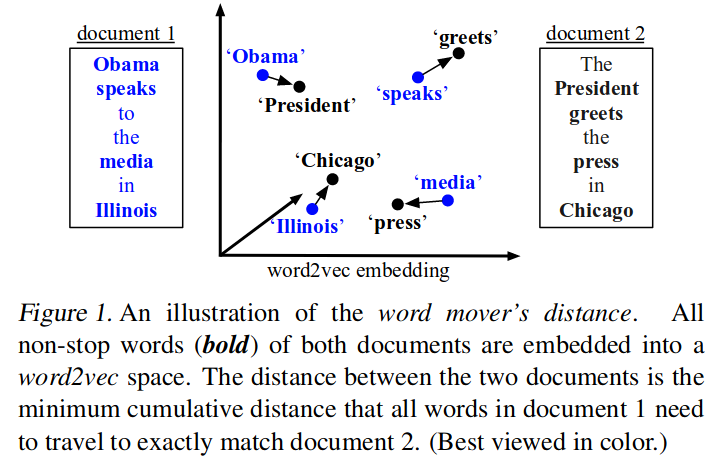
\includegraphics[width=\linewidth,height=\textheight, keepaspectratio]{wmd}}
	
	
\cite{Kusner2015}
\end{frame}


\begin{frame}{There are several approaches}
  \begin{itemize}
  \item word mover's distance
  \item soft cosine similarity
  \end{itemize}
  In common: we use pre-trained embeddings to replace words (that otherwise would just have a random identifier and be unrelated) with vectors representing their meaning, when calculating our measure of interest
\end{frame}


\subsection[Detecting biases]{(Ab-)using word embeddings to detect biases}


\begin{frame}{Biased embeddings \cite{Bolukbasi2016}}
  \begin{itemize}
  \item word embeddings are trained on large corpora
  \item As the task is to learn how to predict a word from its context (CBOW) or vice versa (skip-gram), biased texts produce biased embeddings
  \item If in the training corpus, the words ``man'' and ``computer programmer'' are used in the same context, then we will learn such a gender bias
  \end{itemize}
  
\end{frame}


\begin{frame}{Biased embeddings}
  Usually, we do not want that (and it has a huge potential for a shitstorm)
  
  ~\\
  \pause
  
	unless\ldots
	
	~\\
	\pause
	
	we actually want to chart such biases.
	
\end{frame}


\begin{frame}{An exmaple from our research \parencite{Kroon2021}}
	We trained word embeddings on 3.3 million Dutch news articles.
	
	Are vector representations of outgroups (Maroccans, Muslims) closer to representations of negative stereotype words than ingroups?

\end{frame}


\begin{frame}[plain]
	\makebox[\linewidth]{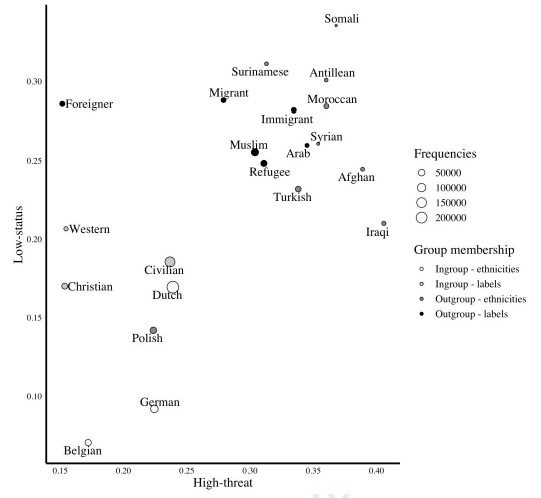
\includegraphics[width=\linewidth,height=\textheight, keepaspectratio]{embeddingbias}}
	
\end{frame}


\subsection[AEM]{AEM: An application from our own research}

\begin{frame}[plain]
	We can use pre-trained embeddings -- but can we make even better ones?
	\textbf{The Amsterdam Embedding Model (AEM)}\\
	
	
	\vspace{1cm}
	
	{\footnotesize{Anne Kroon, Antske Fokkens, Damian Trilling, Felicia Loecherbach, Judith Moeller, Mariken A. C. G. van der Velden, Wouter van Atteveldt} }
\end{frame}



%For all these tasks, you need to process text. 
%Humans are obviously very good in this. However, we are not capable of handling %humongous amounts of data. Therefore, we need computers. 
%For computers, it used to be relatively hard to understand language, to capture %semantic relations, especially in different type of contexts. 


\begin{frame}{Why do this?}
	\begin{itemize}
		\item Embedding models are of great interest to communication scholars
		\item yet... Most publicly available models represent \textbf{English} language
		\item The preparation of good-performing embedding models require a significant amount of \textbf{time} and \textbf{access to a large amount of data sets}
		\item Few Dutch embedding models are available, but trained on ordinary human language from the World Wide Web.
		\item These models do not capture the specifics of news article data and are therefore less suitable to study and understand dynamics of this domain
		\item $\Rightarrow$ No model is available trained on Dutch news data
	\end{itemize}
\end{frame}

%Properly trained embedding models are of great interest to communication scholars, because they can help with diverse tasks, such as topic classification, automated sentiment analysis or bias detection. Yet – currently no model exist that is trained on media data – and therefore effectively deals with the particularities of news media data. 

%\subsection{The Amsterdam Embedding Model}
\begin{frame}{Project's Aim}
	\begin{block}{Aim of the current project} 
		\begin{enumerate}
			\item Develop and evaluate a high-quality embedding model
			\item Assess performance in downstream tasks of interest to Communication Science (such as topic classification of newspaper data).
			\item Facilitate distribution and use of the model
			\item Offer clear methodological recommendations for researchers interested using our Dutch embedding model
		\end{enumerate}
	\end{block}
\end{frame}

%Therefore, this project was set out to develop a good word embedding model trained on Dutch media data, and facilitate its distribution


%\subsection{Approach and Preliminary Results}

\begin{frame}{Training data}
  \begin{block}{Training data set}
    \begin{itemize}
    \item Dataset: diverse print and online news sources
    \item Preprocessing: duplicate sentences were removed
    \item Telegraaf (print \& online), NRC Handelsblad (print \& online), Volkskrant (print \& online), Algemeen Dabldad (print \& online), Trouw (print \& online), nu.nl , nos.nl
    \item \# words: 1.18b (1181701742)
    \item \# sentences: 77.1M (77151321)
    \end{itemize}
  \end{block}
\end{frame}

\begin{frame}{Training model}
  \begin{block}{Training model}
    \begin{itemize}
    \item We trained the model using Gensim's Word2Vec package in Python
    \item Skip-gram with negative sampling, window size of 5, 300-dimensional word vectors
    \end{itemize}
  \end{block}
\end{frame}


\begin{frame}{Evaluation}
  Evaluation of the Amsterdam Embedding Model
\end{frame}

\begin{frame}{Evaluation}
  \begin{block}{Evaluation methods}
    \begin{itemize}
    \item To evaluate the model, we compare it to two other publicly available embedding models
      \begin{itemize}
      \item $\Rightarrow$ \textbf {'Wiki'}: Embedding model trained on Wikipedia data (FastText)
      \item $\Rightarrow$ \textbf{'Cow'}: Embedding model trained on diverse .nl and .be sites (Schafer \& Bildhauer, 2012; Tulkens et al., 2016)
      \item $\Rightarrow$ \textbf{'AEM'}: Amsterdam Embedding Model
      \end{itemize}
    \end{itemize}
  \end{block}
\end{frame}

%To evaluate our model, we will compare it (at least in a first step) – to two other, publicly available word embedding models: One trained on Wikipedia data, and the other on divers dutch and Belgian websites. 

\begin{frame}{Evaluation data}
  \begin{block}{Evaluation data}
    \begin{enumerate}
    \item 'relationship'/ analogy-task (Tulkens et al., 2016)
      \begin{itemize}
      \item \textbf{syntatic relationships}: dans dansen loop \textit{[lopen]}
      \item \textbf{semantic relationships}: denemarken kopenhagen noorwegen \textit{[oslo]}
      \end{itemize}
    \item 5806 relationship tasks
    \end{enumerate}
  \end{block}
\end{frame}

%Tulkens et al created several Dutch relationship tasks. For example, when given dans (dance) dansen (dancing) and loop (walk), the computer has to guess that the word we are looking for is lopen (walking). This is an example of syntactic analogy. The same applies to capital - country relations (Copenhagen is to Denmark as … [Oslo] to Norway]. This is an example of a semantic analogy. 
%Each model had to solve over 5K of these types of analogy tasks. We subsequently use these results to compare how well they do.

\begin{frame}{}
	\makebox[\linewidth]{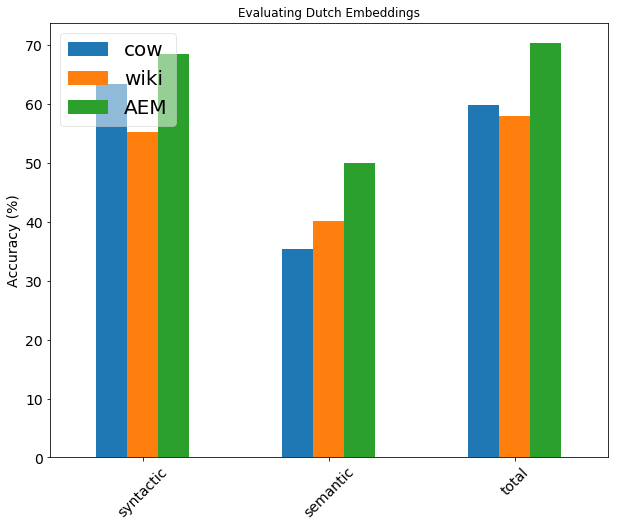
\includegraphics[width=\linewidth,height=\textheight, keepaspectratio]{evaluation_data.png}}
\end{frame}





\begin{frame}{}
	\makebox[\linewidth]{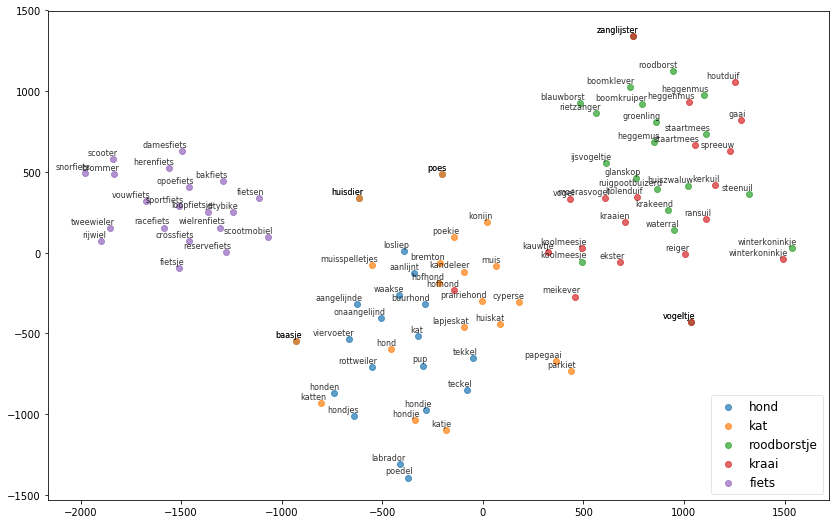
\includegraphics[width=\linewidth,height=\textheight, keepaspectratio]{aem-w2v_300_illustration.png}}
\end{frame}

% this is a 2 dimensional representation of the most similar words to fiets, hond, kat, roodborstje and kraai 

\begin{frame}{}
	\makebox[\linewidth]{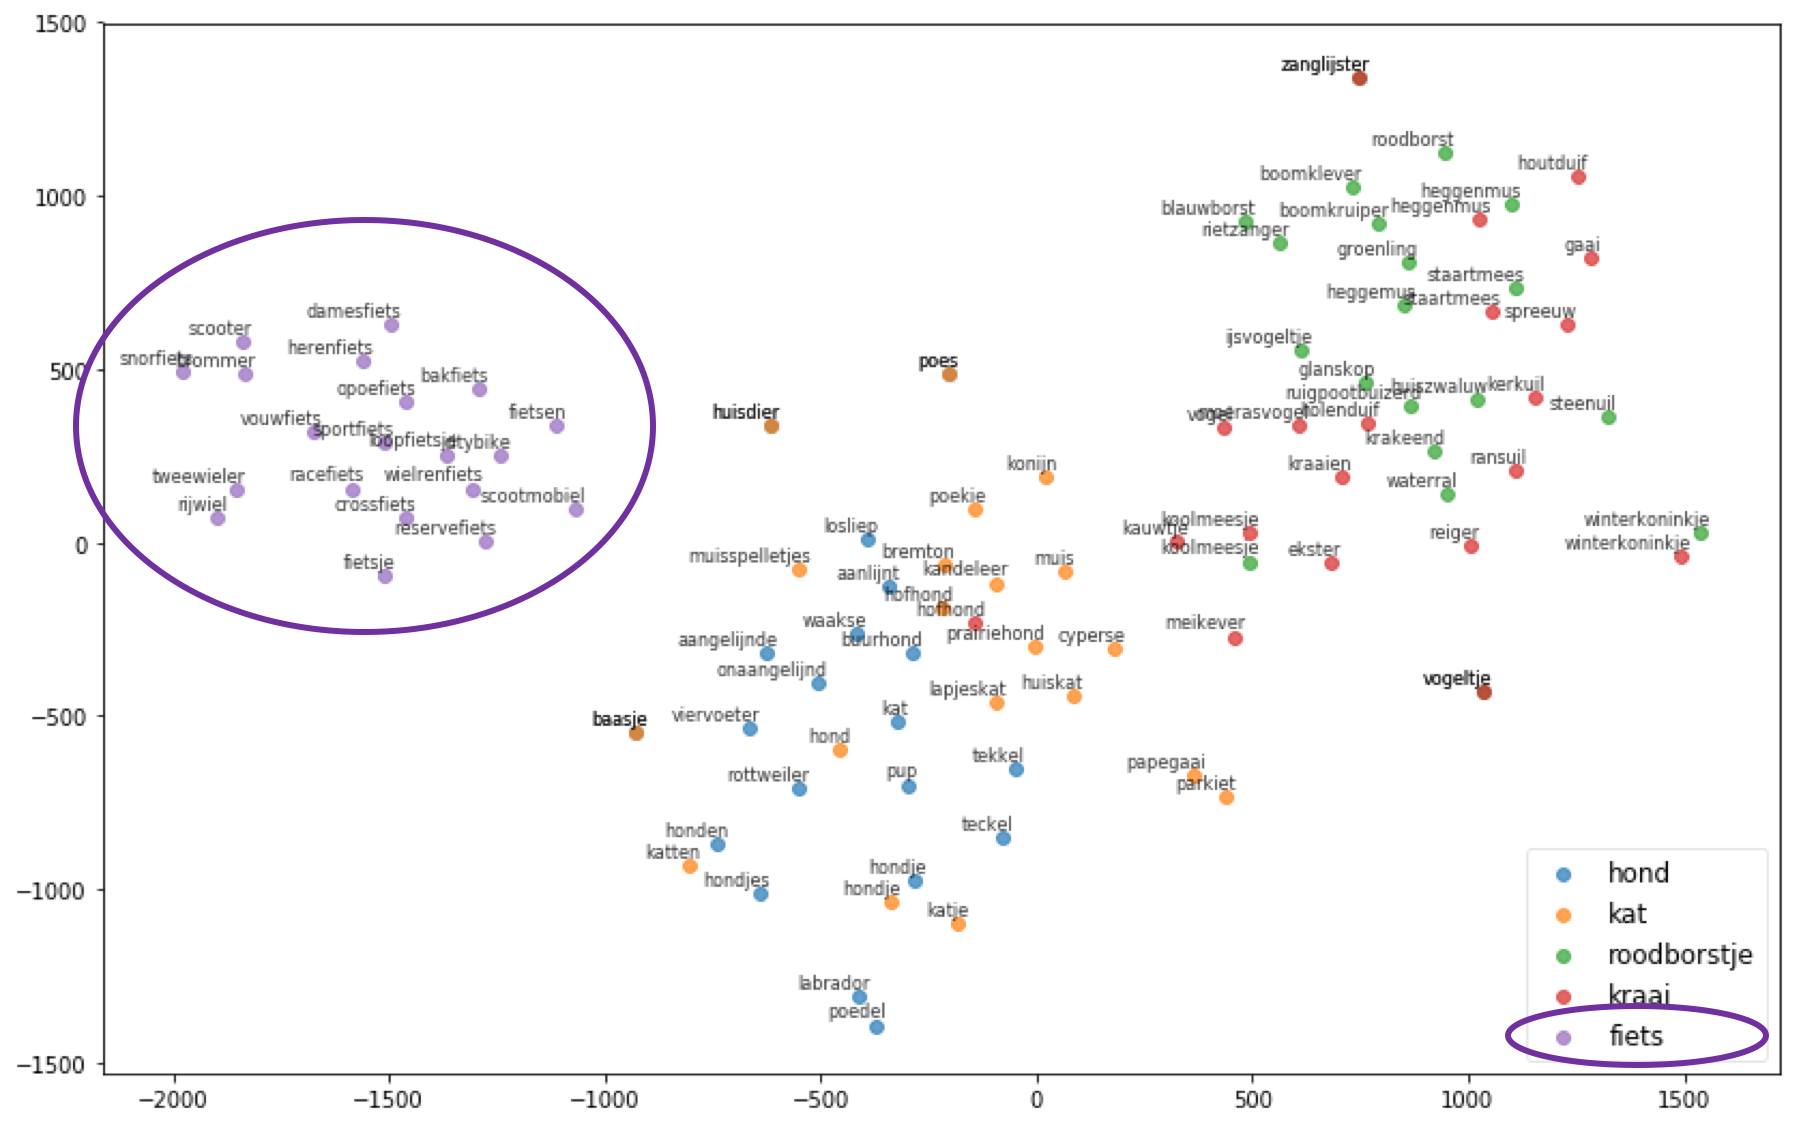
\includegraphics[width=\linewidth,height=\textheight, keepaspectratio]{aem-visual2.png}}
\end{frame}

%as can be seen, words most similar to fiets are on the left. 

\begin{frame}{}
	\makebox[\linewidth]{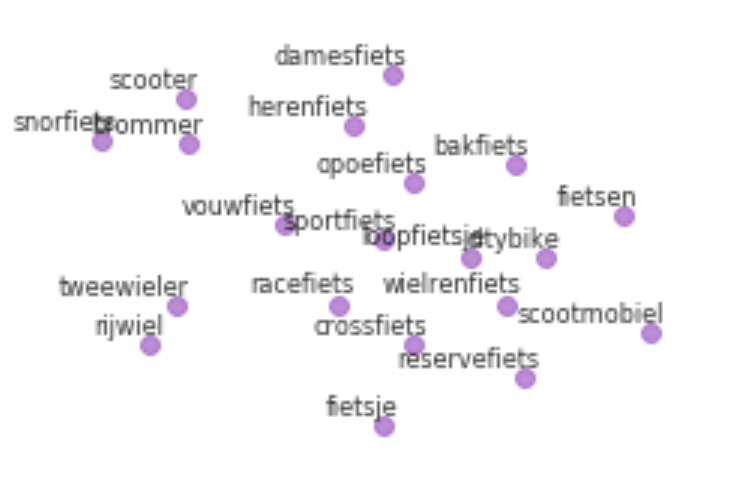
\includegraphics[width=\linewidth,height=\textheight, keepaspectratio]{aem-fiets}}
\end{frame}

%the model has learned that fiets is similar to racefiets, wielrenfiets, rijwiel - and different from the animal department: it doesnt overlap with our kats/ dogs and birds clusters

\begin{frame}{}
	\makebox[\linewidth]{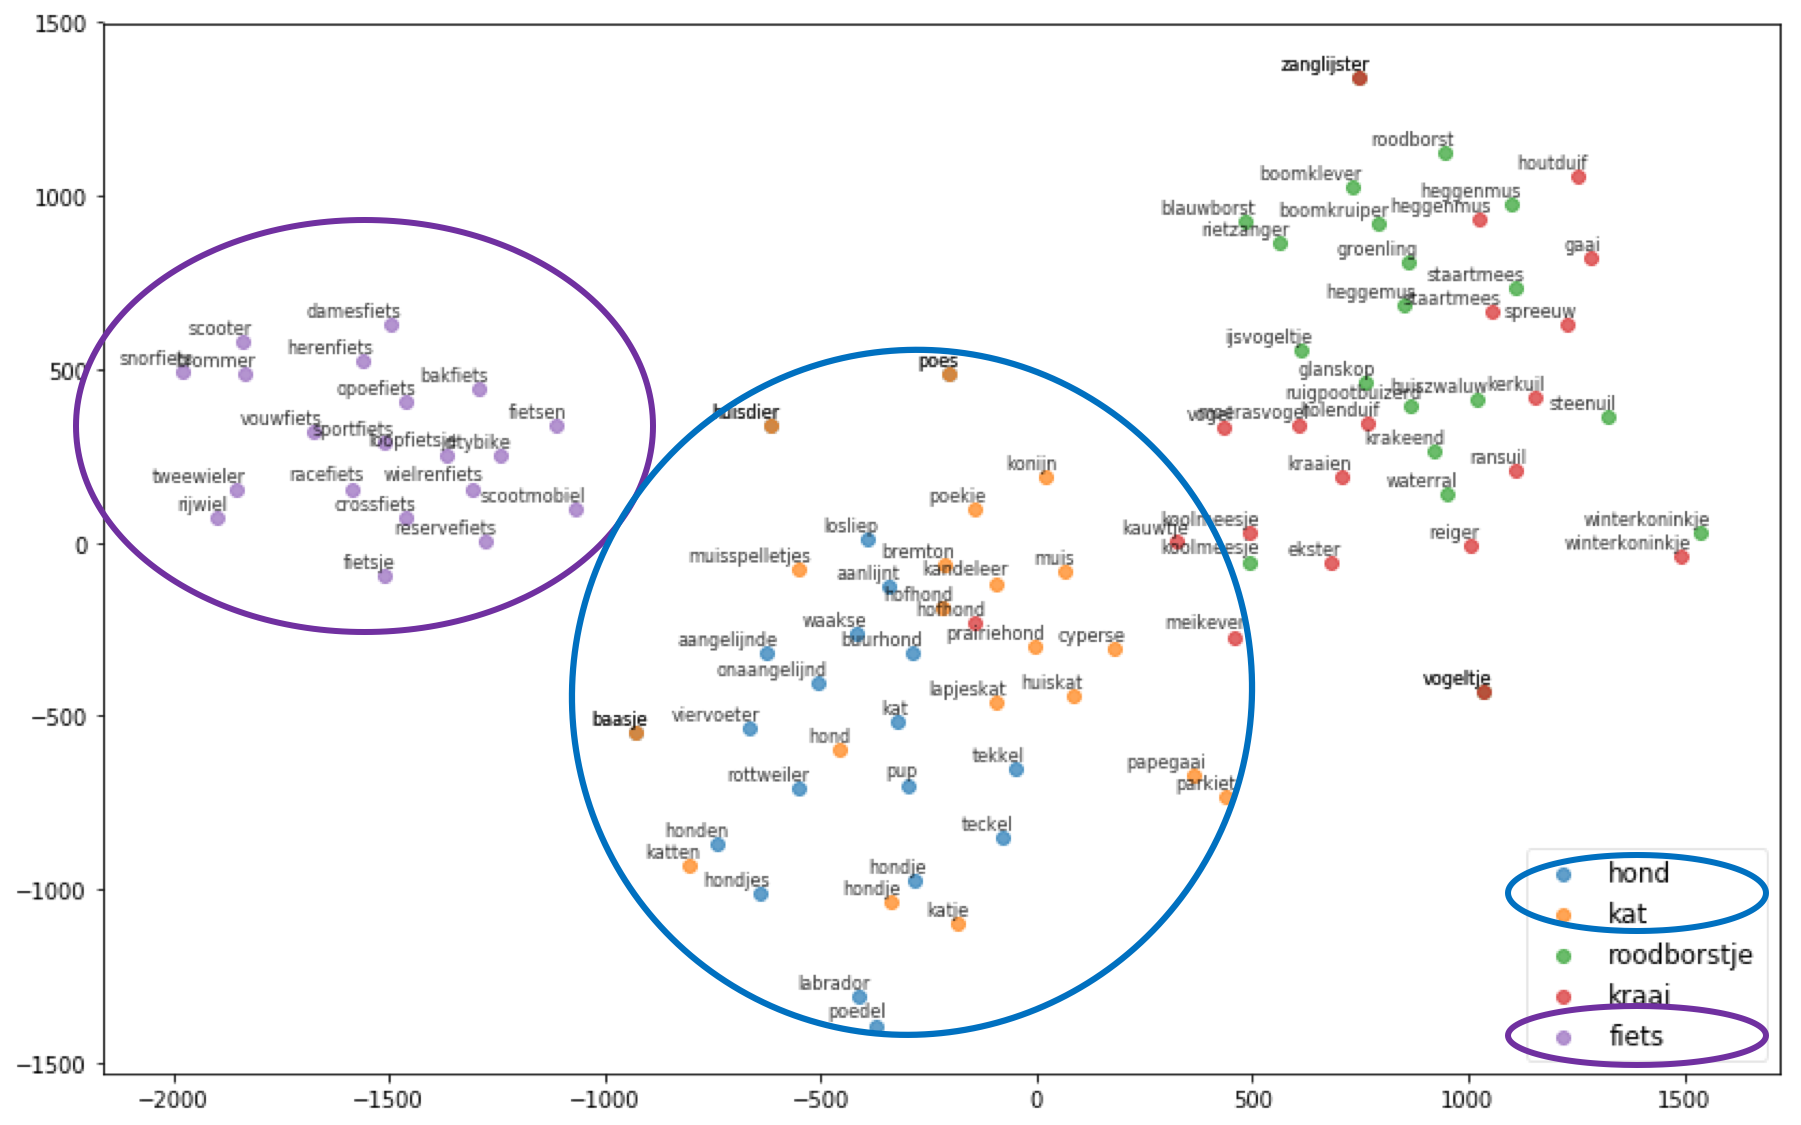
\includegraphics[width=\linewidth,height=\textheight, keepaspectratio]{aem-visual1.png}}
\end{frame}

%the model recognizes that fiets is something else from honden and katten. Both mammals and pets, dogs and cats are quite similar and appear in the same cluster.  

\begin{frame}{}
	\makebox[\linewidth]{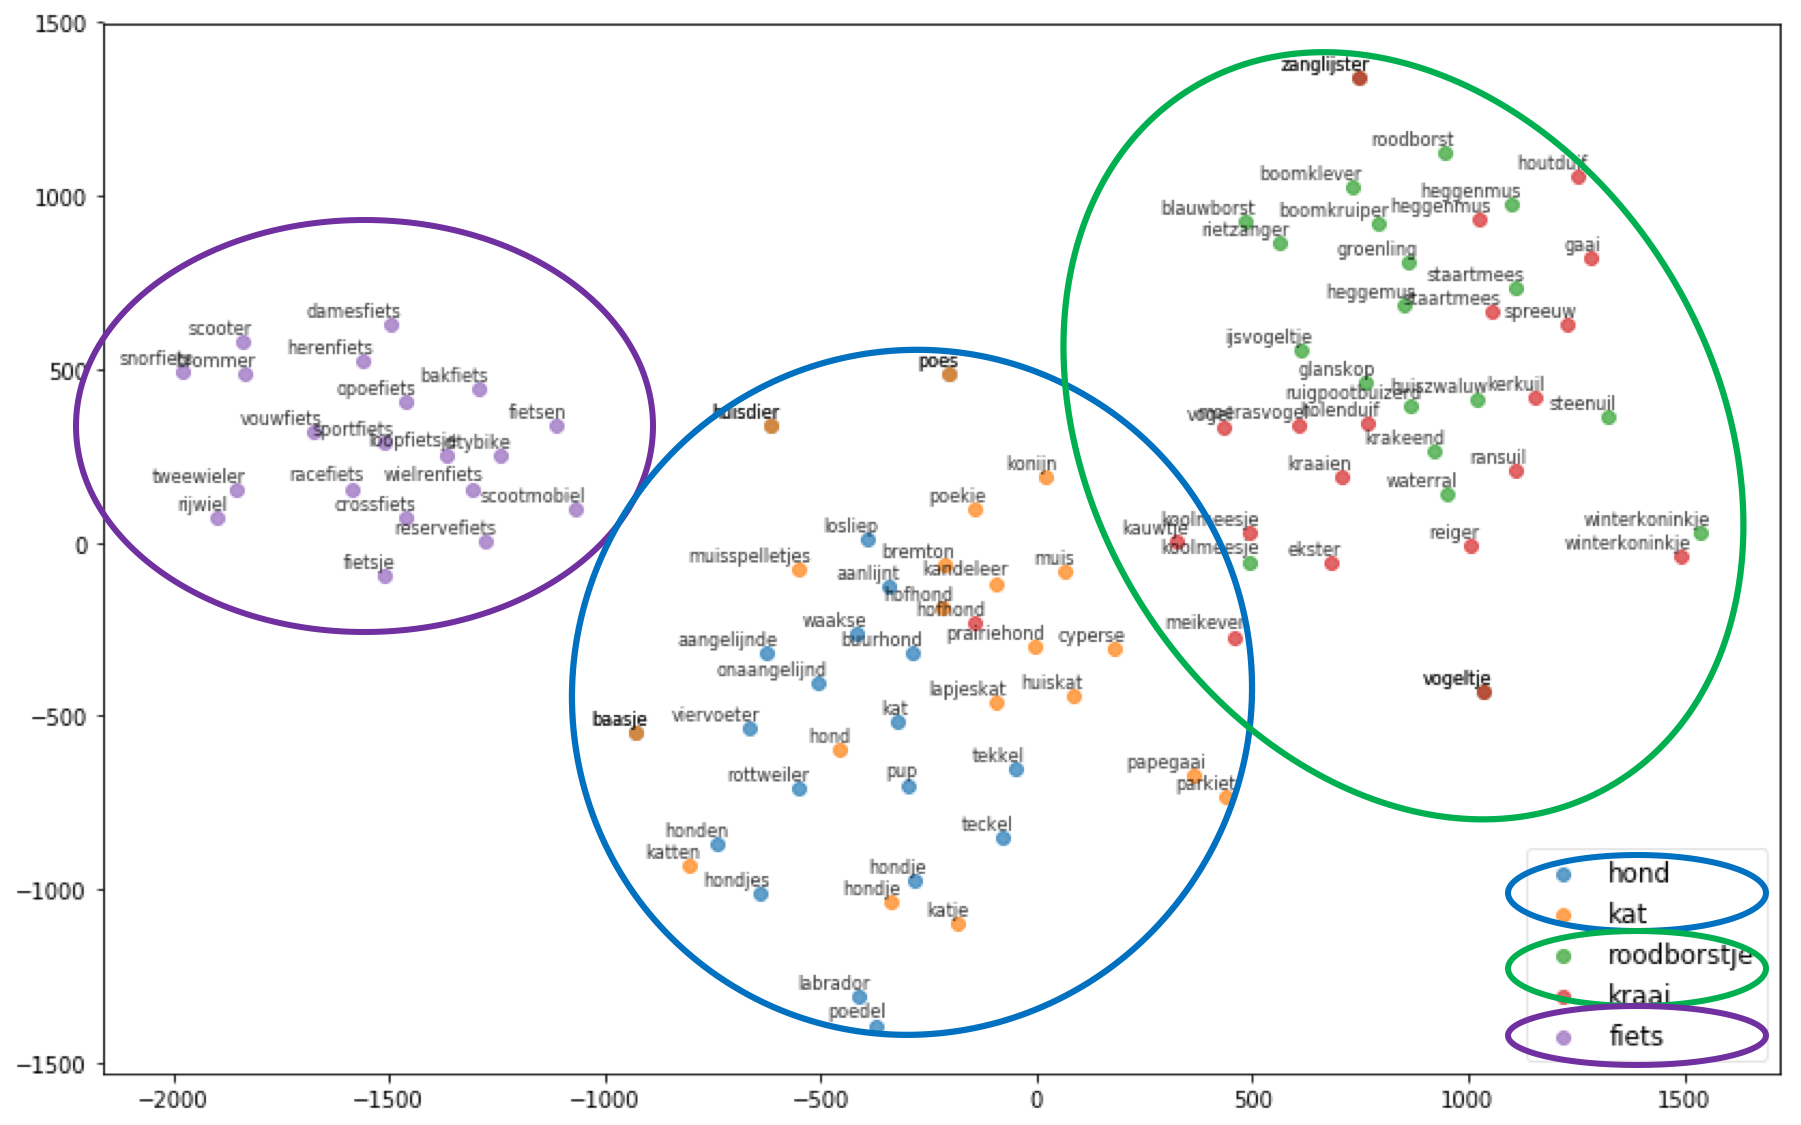
\includegraphics[width=\linewidth,height=\textheight, keepaspectratio]{aem-visual.png}}
\end{frame}

%Finally, the model recognizes that dogs and kats are different from redbreasts and crows, with both appear in a 'bird-related' cluster.

%\begin{frame}{}
%	\makebox[\linewidth]{\includegraphics[width=\linew%idth,height=\textheight, %keepaspectratio]{bias.png}}
%\end{frame}

%Now we know that the model understands Dutch pretty well. We can now apply to model to diverse tasks that are of greater interest to communication scholars. For example, we can see whether or not our training data contains bias.When we plot the most similar words to ‘criminals, Belgians and Moroccans,  we see that Moroccans are much closer to criminals, that Belgians. THis could potentiall reveal bias in the training data.

%\subsection{Re-usability}
\begin{frame}{Re-usability}
	Re-usability of the Amsterdam Embedding Model
\end{frame}

%\subsection{Availability of model and code}
\begin{frame}{Re-usability}
  \begin{block}{Reusing model and data}
    \begin{enumerate}
    \item See \url{https://github.com/annekroon/amsterdam-embedding-model}
    \item Open access to all the code
    \end{enumerate}
  \end{block}
\end{frame}



\subsection{Downstream tasks}


\begin{frame}{Document comparison: An example \parencite{Trilling2021}}
  Let's say we have a large corpus of news articles and what to find those that are about the same events.
  
\end{frame}


\begin{frame}{Data}
  \begin{itemize}
  \item 45K articles
  \item 6 months
  \item volkskrant.nl, ad.nl, nu.nl
  \end{itemize}
\end{frame}



\begin{frame}{Step 1: Get candidate articles}
  Comparing everything with everything is
  \begin{itemize}
  \item computationally infeasible
  \item theoretical nonsensical
  \end{itemize}
  
  \begin{block}{Our solution}
    \begin{itemize}
    \item Three-day moving window (but ``chaining'' possible)
    \item  Saturday/Sunday merged into one day
    \end{itemize}
  \end{block}
  
\end{frame}




\begin{frame}{Step 2: Get similarity scores}
  How to determine similarity between articles?
  \begin{block}{Our solution}
  Compare combinations of 
  \begin{itemize}
  \item different measures (in particular, $tf\cdot idf$ cosine similarity vs. softcosine similarity
  \item different thresholds (to get rid of the overwhelming majority of close-to-zero edges) 
  \end{itemize}
\end{block}
\end{frame}


\begin{frame}{Step 3: Network clustering}
  How to determine events?

  After experimenting \emph{a lot}:
	
  \begin{block}{Our final solution}
    \begin{itemize}
    \item One network for all (instead of one per window)
    \item Articles are nodes, similarity scores = edge weights
    \item all edges with weight $<$ threshold removed
    \item Leiden algorithm (\cite{Traag2019}) with Surprise method (\cite{Traag2015}) (very suitable for smaller, but more clusters)
    \end{itemize}
  \end{block}
  
\end{frame}


\begin{frame}{Number of articles per event}
\begin{table}[h]
  \caption{Descriptives for different threshold/similarity combinations\label{tab:thresholds}}
  
  \centering
  \resizebox{\textwidth}{!}{%
    \begin{tabular}{lrrrrr|rrrrr}
      \toprule
	  {} & \multicolumn{5}{c}{\textbf{cosine}} & \multicolumn{5}{c}{\textbf{softcosine}} \\
	  {} &    0.2  & 0.3 & 0.4 & 0.5 & 0.6 & 0.2 & 0.3  & 0.4 & 0.5 & 0.6  \\
	  \midrule
	  mean              &  2.03 & 1.58 & 1.35 & 1.21 & 1.12 & 6.78 & 2.89 & 1.88 & 1.51  & 1.27 \\
	  std              &  3.48 & 2.00 & 1.22 & 0.71 & 0.45  & 30.41 & 10.04 & 4.27 & 2.27 & 1.07 \\
	  max              &   88 & 53 & 41 & 21   & 15 & 551 & 367 & 161 & 70 & 30  \\
	  single-art.\\ events & 15626  & 21854  & 27135 & 32232 & 36348 & 4262 & 11043 & 18305 & 24337 & 30700 \\
	  multi-art.\\ events & 6685 & 6777 & 6241 & 5165 & 3899 & 2460 & 4736 & 5961 & 5940 & 5257 \\
	  \bottomrule
    \end{tabular}
  }%
\end{table}
\end{frame}



\begin{frame}{What does that mean?}
  \begin{itemize}
  \item Use a high threshold!
  \item Soft-cosine finds some more events, leaves less articles unassigned (good), but that comes at the expense of slightly lower precision
  \item Example from our data: Because soft-cosine ``understands'' that Nike and Puma are both sports brands, it incorrectly assigned economic coverage about the two to one event.
  \end{itemize}
\end{frame}




\begin{frame}[fragile]{How correct are the events?}
  We manually checked $6 \times 100$ events, qualitatively (not shown) and quantitatively:
  \begin{table}
    \begin{tabular}{lrrrr}
      \footnotesize
      \textbf{Similarity}   & \textbf{Threshold} & \textbf{Prec. 1 (\%)} & \textbf{Prec. 2 (\%)} &\textbf{TP/max. TP}  \\
      \midrule
      cosine              & 0.4       & 74        & 88.52     & 223/268 \\
      cosine              & 0.5       & 78        & 89.02     & 217/253 \\
      cosine              & 0.6       & 89        & 94.39     & 204/225 \\
      softcosine          & 0.4       & 56        & 76.20     & 234/521 \\
      softcosine          & 0.5       & 65        & 81.77     & 236/379 \\
      softcosine          & 0.6       & 75        & 86.92     & 222/289 \\
      
    \end{tabular}
	\end{table}
	\tiny 
	\textit{Note.} \textit{Precision 1:} The percentage of news events that are entirely clustered correctly. \textit{Precision 2:} The percentage of news articles that are correctly clustered. \textit{max. TP} is the number of articles that are assigned to an event in the sample; hence, the maximum number of true positives that can be achieved.\\
	
\end{frame}

\begin{frame}{Cosine vs Softcosine}
	Also a matter of computational costs
	\begin{itemize}
	\item the document needs to be converted into embeddings
	\item but once that is done, our document vectors only have 300 instead of thousands of dimensions!
	\end{itemize}
\end{frame}

